\documentclass[aps,secnumarabic,amsmath,amssymb,superscriptaddress]{revtex4}
\usepackage{amsmath}
\usepackage{amssymb}
\usepackage{amsfonts}
\usepackage{color}
\usepackage{graphics}
\usepackage[pdftex]{graphicx}
\usepackage[utf8x]{inputenc}
\usepackage[colorlinks=true]{hyperref}
\usepackage{listings}
\usepackage{braket}

\newcommand{\ud}{\mathrm{d}}
\newcommand{\ue}{\mathrm{e}}
\newcommand{\ui}{\mathrm{i}}
\newcommand{\res}{\mathrm{Res}}
\newcommand{\Tr}{\mathrm{Tr}}
\newcommand{\dsum}{\displaystyle\sum}
\newcommand{\dprod}{\displaystyle\prod}
\newcommand{\dlim}{\dispqlaystyle\lim}
\newcommand{\dint}{\displaystyle\int}
\newcommand{\fsno}[1]{{\!\not\!{#1}}}
\newcommand{\texp}[2]{\ensuremath{{#1}\times10^{#2}}}
\newcommand{\dexp}[2]{\ensuremath{{#1}\cdot10^{#2}}}
\newcommand{\eval}[2]{{\left.{#1}\right|_{#2}}}
\newcommand{\paren}[1]{{\left({#1}\right)}}
\newcommand{\lparen}[1]{{\left({#1}\right.}}
\newcommand{\rparen}[1]{{\left.{#1}\right)}}
\newcommand{\abs}[1]{{\left|{#1}\right|}}
\newcommand{\sqr}[1]{{\left[{#1}\right]}}
\newcommand{\crly}[1]{{\left\{{#1}\right\}}}
\newcommand{\angl}[1]{{\left\langle{#1}\right\rangle}}
\newcommand{\tpdiff}[4][{}]{{\paren{\frac{\partial^{#1} {#2}}{\partial {#3}{}^{#1}}}_{#4}}}
\newcommand{\tpsdiff}[4][{}]{{\paren{\frac{\partial^{#1}}{\partial {#3}{}^{#1}}{#2}}_{#4}}}
\newcommand{\pdiff}[3][{}]{{\frac{\partial^{#1} {#2}}{\partial {#3}{}^{#1}}}}
\newcommand{\diff}[3][{}]{{\frac{\ud^{#1} {#2}}{\ud {#3}{}^{#1}}}}
\newcommand{\psdiff}[3][{}]{{\frac{\partial^{#1}}{\partial {#3}{}^{#1}} {#2}}}
\newcommand{\sdiff}[3][{}]{{\frac{\ud^{#1}}{\ud {#3}{}^{#1}} {#2}}}
\newcommand{\tpddiff}[4][{}]{{\left(\dfrac{\partial^{#1} {#2}}{\partial {#3}{}^{#1}}\right)_{#4}}}
\newcommand{\tpsddiff}[4][{}]{{\paren{\dfrac{\partial^{#1}}{\partial {#3}{}^{#1}}{#2}}_{#4}}}
\newcommand{\pddiff}[3][{}]{{\dfrac{\partial^{#1} {#2}}{\partial {#3}{}^{#1}}}}
\newcommand{\ddiff}[3][{}]{{\dfrac{\ud^{#1} {#2}}{\ud {#3}{}^{#1}}}}
\newcommand{\psddiff}[3][{}]{{\frac{\partial^{#1}}{\partial{}^{#1} {#3}} {#2}}}
\newcommand{\sddiff}[3][{}]{{\frac{\ud^{#1}}{\ud {#3}{}^{#1}} {#2}}}
\newcommand{\eff}{ef\! f}

\newcommand{\todo}[1]{}

\newcommand{\harvardphysics}{\affiliation{Department of Physics, Harvard University, Cambridge, Massachusetts 02138, USA}}
\newcommand{\harvardccb}{\affiliation{Department of Chemistry and Chemical Biology, Harvard University, Cambridge, Massachusetts 02138, USA}}
\newcommand{\cua}{\affiliation{Harvard-MIT Center for Ultracold Atoms, Cambridge, Massachusetts 02138, USA}}
\newcommand{\gradstudent}{
  \harvardphysics
  \harvardccb
  \cua
}

% Add S1 to bibliography
\bibliographystyle{apsrev4-2}
\renewcommand*{\citenumfont}[1]{S#1}
\renewcommand*{\bibnumfmt}[1]{[S#1]}

% Add S to labels
\setcounter{table}{0}
\renewcommand{\thetable}{S\arabic{table}}%
\setcounter{figure}{0}
\renewcommand{\thefigure}{S\arabic{figure}}%
\renewcommand{\thepage}{S\arabic{page}}
\renewcommand{\thesection}{S\arabic{section}}
\renewcommand{\theequation}{S.\arabic{equation}}

\ifpdf
% Ensure reproducible output
\pdfinfoomitdate=1
\pdfsuppressptexinfo=-1
\pdftrailerid{}
\hypersetup{
  pdfcreator={},
  pdfproducer={}
}
\fi

\begin{document}
\title{Coherent optical association of a single molecule -- Supplemental material}
\author{Yichao~Yu}
\email{yichaoyu@g.harvard.edu}
\gradstudent
\author{Kenneth~Wang}
\gradstudent
\author{Jonathan~D.~Hood}
\affiliation{Department of Chemistry, Purdue University, West Lafayette, Indianna, 47906}
\author{Lewis~R.~B.~Picard}
\gradstudent
\author{Jessie~T.~Zhang}
\gradstudent
\author{William~B.~Cairncross}
\harvardccb
\harvardphysics
\cua
\author{Jeremy~M.~Hutson}
\affiliation{Joint Quantum Centre Durham-Newcastle, Department of Chemistry, Durham University, Durham, DH1 3LE, United Kingdom}
\author{Till Rosenband}
\harvardphysics
\author{Kang-Kuen~Ni}
\email{ni@chemistry.harvard.edu}
\harvardccb
\harvardphysics
\cua

\date{\today}

\maketitle

\section{3 Level Raman Transfer with Cross Coupling}

In our system, the separation in energy between the initial and target state is much smaller than the single photon detuning $\Delta$ from the intermediate state. Thus, there is significant cross coupling for the scattering rate and light shift, where each state is coupled to the excited state by the power in both beams. Under these conditions, the scattering rate and light shift is proportional to the total power $P_{\text{tot}} = P_m + P_a$, where $P_{m} (P_{a})$ is the power in the beam that addresses the molecular (atomic) state. The Raman Rabi frequency is proportional to $\sqrt{P_mP_a} $. With a fixed total power and thus fixed scattering rate, the Raman Rabi frequency is maximized when $ P_m = P_a = P_{\text{tot}}/2$.

For the purposes of this work, we denote $\Omega_a $($\Omega_m$) as the Rabi frequencies to drive a transition from the atom (target molecule) state to the intermediate state used in the Raman transition corresponding to the power in a single beam, $P_a$ ($P_m$). Thus, the Raman Rabi frequency is $\Omega_a\Omega_m/2\Delta$, where $ \Delta $ is the single photon detuning. Cross coupling affects the scattering rate and light shift, and assuming equal powers in both beams, these quantities become $ \Gamma_e \Omega_m^2 / 2\Delta^2 + \Gamma_e \Omega_a^2 / 2\Delta^2 $ and $ \Omega_m^2/2\Delta - \Omega_a^2/2\Delta $, where $\Gamma_e$ is the excited state linewidth. Since $ \Omega_m >> \Omega_a $, the scattering rate and light shift can be approximated as $ \Gamma_e \Omega_m^2/2\Delta^2$ and $\Omega_m^2/2\Delta$.

\section{Raman Transfer with Many Intermediate States} \label{sm:sect_2}
With multiple intermediate states, the total Raman Rabi frequency, scattering rate, and light shift become a sum over all these possible states. In our model, we consider all vibrational states of $ \mathrm{c^3\Sigma^+(\Omega = 1)} $ and states in the atomic continuum as intermediate states. The Rabi frequency between two states is proportional to the electronic dipole moment, arising from the electronic wavefunctions, and the overlap of the vibrational wavefunctions. Under the assumption that the electronic dipole moment $ d $ is the same for all transitions between the ground state and the excited electronic state, the total Raman Rabi frequency becomes:

\begin{equation}
  \Omega_R = \frac{d^2E^2}{2\hbar^2} \displaystyle\sum_{v'} \frac{\braket{a|v'}\braket{v'|m}}{\Delta_{v'}}
\end{equation}

where $\ket{a}$ ($\ket{m}$) are the relative coordinate wavefunctions for the trapped atomic (target molecular) state, and $\ket{v'}$ is the relative-coordinate wavefunction for the excited state which includes both bound molecular states and the atomic continuum. $\Delta_{v'}$ is a single photon detuning with respect to the $\ket{v'}$ state, $ E $ is the electric field for the power in the single beam given a waist size. We can divide this sum into a sum over all the bound molecular states, and a sum over atomic continuum states.

\begin{equation}
  \Omega_R = \frac{d^2E^2}{2\hbar^2}\displaystyle\sum_{v' \leq v'_{\text{max}}} \frac{\braket{a|v'}\braket{v'|m}}{\Delta_{v'}} +  \frac{d^2E^2}{2\hbar^2}\displaystyle\sum_{v' > v'_{\text{max}}} \frac{\braket{a|v'}\braket{v'|m}}{\Delta_{v'}}
\end{equation}

where $ v'_{\text{max}}$ corresponds to the excited molecular state, which is most weakly bound. The first term can be calculated numerically given an excited state potential. To calculate the second term, we first make an assumption that we are far enough detuned from the contributing continuum states that they are all at approximately the same detuning, $ \delta_{\text{thresh}}$. This allows us to pull it out of the sum, and we obtain:

\begin{equation}
  \Omega_R \approx \frac{d^2E^2}{2\hbar^2}\displaystyle\sum_{v' \leq v'_{\text{max}}} \frac{\braket{a|v'}\braket{v'|m}}{\Delta_{v'}} +  \frac{d^2E^2}{2\hbar^2\delta_{\text{thresh}}}\displaystyle\sum_{v' > v'_{\text{max}}} \braket{a|v'}\braket{v'|m}  \label{rabifreq}
\end{equation}

From requiring orthogonality,

\begin{equation}
  \displaystyle\sum_{v'} \braket{a|v'}\braket{v'|m} = \braket{a|m} = 0
\end{equation}

we derive an expression for the second sum in equation \ref{rabifreq}

\begin{equation}
  \displaystyle\sum_{v'> v'_{\text{max}}} \braket{a|v'}\braket{v'|m} = -\displaystyle\sum_{v' \leq v'_{\text{max}}} \braket{a|v'}\braket{v'|m}
\end{equation}

which can be calculated from the vibrational states of the excited state potential. Thus, the Raman Rabi frequency can be approximated as:

\begin{equation}
  \Omega_R \approx \frac{d^2E^2}{2\hbar^2}\displaystyle\sum_{v' \leq v'_{\text{max}}} \frac{\braket{a|v'}\braket{v'|m}}{\Delta_{v'}} -  \frac{d^2E^2}{2\hbar^2\delta_{\text{thresh}}}\displaystyle\sum_{v' \leq v'_{\text{max}}} \braket{a|v'}\braket{v'|m}
\end{equation}

We can account for the atomic continuum in the scattering rate in a similar way.

\begin{align}
  \Gamma_s &= \frac{d^2E^2}{2\hbar^2}\displaystyle\sum_{v' \leq v'_{\text{max}}}\Gamma_{v'} \frac{\braket{m|v'}\braket{v'|m}}{\Delta_{v'}^2} + \frac{d^2E^2}{2\hbar^2}\displaystyle\sum_{v' > v'_{\text{max}}}\Gamma_{v'} \frac{\braket{m|v'}\braket{v'|m}}{\Delta_{v'}^2} \\
           &\approx \frac{d^2E^2}{2\hbar^2}\displaystyle\sum_{v' \leq v'_{\text{max}}}\Gamma_{v'} \frac{\braket{m|v'}\braket{v'|m}}{\Delta_{v'}^2} + \frac{d^2E^2\Gamma}{2\hbar^2\delta_{\text{thresh}}^2}\displaystyle\sum_{v' > v'_{\text{max}}}\braket{m|v'}\braket{v'|m}
\end{align}

where $\Gamma_{v'}$ is the excited state linewidth for the $\ket{v'}$ state, and we have assumed the atomic continuum states all have the same linewidth $\Gamma$. Using normalization, we derive an expression for the sum in the second term

\begin{equation}
  \displaystyle\sum_{v' > v'_{\text{max}}}\braket{m|v'}\braket{v'|m} = 1 - \displaystyle\sum_{v' \leq v'_{\text{max}}}\braket{m|v'}\braket{v'|m}
\end{equation}

We then arrive at an expression for the scattering rate, accounting for the atomic continuum,

\begin{equation}
  \Gamma_s \approx \frac{d^2E^2}{2\hbar^2}\displaystyle\sum_{v' \leq v'_{\text{max}}}\Gamma_{v'} \frac{\braket{m|v'}\braket{v'|m}}{\Delta_{v'}^2} +  \frac{d^2E^2\Gamma}{2\hbar^2\delta_{\text{thresh}}^2}\left(1 - \displaystyle\sum_{v' \leq v'_{\text{max}}}\braket{m|v'}\braket{v'|m}\right)
\end{equation}

The effect of the continuum is to add an extra state at the atomic threshold with strength proportional to the amount of wavefunction overlap between the target-molecular state and all atomic continuum states. This term is especially important for our target-molecule state, because the square of the wavefunction overlap between the target-molecule state and all excited vibrational states is only 0.02

\begin{equation}
  \displaystyle\sum_{v' \leq v'_{\text{max}}}\braket{m|v'}\braket{v'|m} = 0.02
\end{equation}

leading to strong scattering from the atomic continuum. We note that this model leads to a component in the scattering rate that is proportional to $ 1/\delta_{\text{thresh}}^2$ and is smaller as one detunes farther from the threshold.

A very similar result holds for the light shift and is written here for completeness

\begin{equation}
  \frac{d^2E^2}{2\hbar^2}\displaystyle\sum_{v' \leq v'_{\text{max}}} \frac{\braket{m|v'}\braket{v'|m}}{\Delta_{v'}} +  \frac{d^2E^2}{2\hbar^2\delta_{\text{thresh}}}\left(1 - \displaystyle\sum_{v' \leq v'_{\text{max}}}\braket{m|v'}\braket{v'|m}\right)
\end{equation}


\section{Calculating Matrix Elements with Coupled Channel Ground State}
The free atom state (with spherically-symmetric harmonic confinement) and target weakly-bound molecular state are calculated using coupled-channel methods. With the cylindrical symmetry present at non-zero magnetic field, the magnetic quantum number is a good quantum number. We use the spin combination $ \ket{F_{\text{Na}} = 2, m_{F_{\text{Na}}} = 2, F_{\text{Cs}} = 3, m_{F_{\text{Cs}}} = 3}$, so channels with total $ m_F = 5 $ are included. These channels, written in the basis $ \ket{S, m_S, I, m_I}$, include $ \ket{0,0,5,5}, \ket{1,0,5,5}, \ket{1,1,5,4}, \ket{1,1,4,4} $, where $S = 0,1$ is the total electron spin and $ I = 2,3,4,5 $ is the total nuclear spin. For each of these channels, there is a different vibrational wavefunction. In this work, we assume the excited state wavefunction is a single-channel wavefunction, so that it is purely triplet. Thus, only the triplet component of the coupled-channel ground state wavefunction contributes to $\Omega_a$ and $ \Omega_m $.

The full calculation using the methods in section \ref{sm:sect_2} is shown in figure \ref{f-sm}. The strong contribution from the atomic threshold arises from the large overlap between the weakly-bound molecular state and the atomic continuum. This leads to a $1/\delta_{\text{thresh}}^2$ dependence of the scattering rate and favors deeply bound states as the intermediate state. The Raman Rabi frequency is larger than the scattering rate only for these deeply bound states.

\begin{figure}[ht!]
  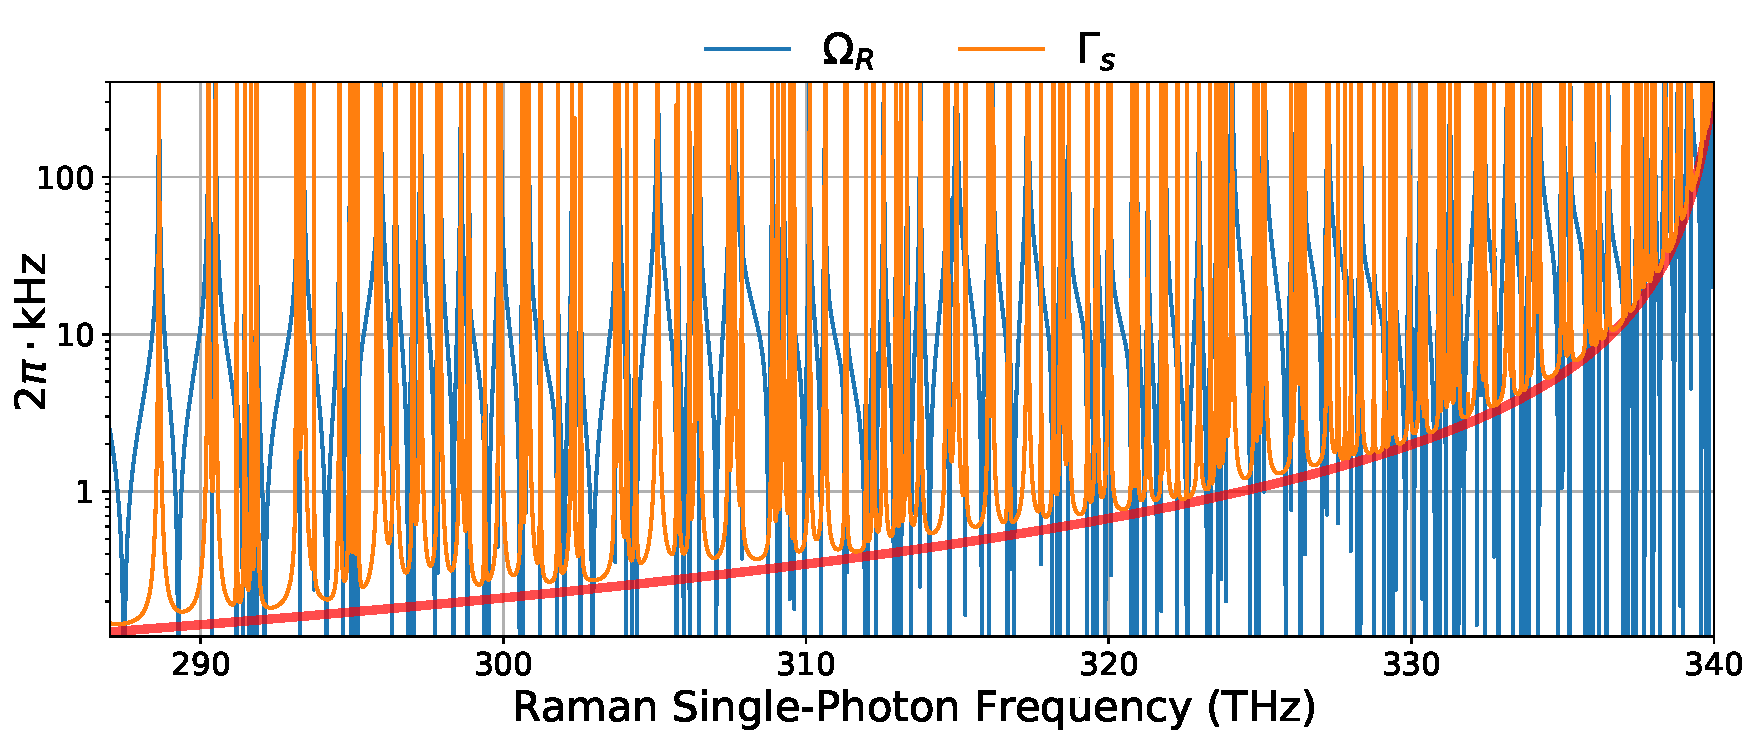
\includegraphics[width=\textwidth]{imgs/raman_theory_full.pdf}
  \caption{ Full calculation of the Raman Rabi frequency and scattering rate as a function of the single-photon frequency including all vibrational states of $ \mathrm{c^3\Sigma^+(\Omega = 1)}$ and the atomic continuum. The second frequency in the Raman transition is offset by about $770~\mathrm{MHz}$ and resonant with the two photon transition. The assumed excited-state linewidth for all molecular lines is $20~\text{MHz} $.
    \label{f-sm}}
\end{figure}


Since our coupled-channel calculations include the harmonic confinement, we can calculate the enhancement in $\Omega_a$ with increasing confinement. Using two calculations with $ \omega_{\text{trap}} = 36.5~\mathrm{kHz}$ and $\omega_{\text{trap}} = 80~\mathrm{kHz}$ trapping frequencies, and assuming a power law scaling, we find $ \Omega_a \propto \omega_{\text{trap}}^{0.58} $. Thus, $\Omega_a \propto P^{0.29} $, which was also experimentally verified. However, we note that in the actual experiment, our system does not have spherically symmetric confinement. The radial trapping frequency is about $5.7$ times larger than the axial trapping frequency.
\todo{
  Power/intensity calibration
}

\bibliography{master_ref}
\end{document}
